\documentclass{beamer}
\usetheme[numbering=fullbar,%nofirafonts
]{focus}
\definecolor{main}{RGB}{92, 138, 168}
\definecolor{background}{RGB}{255,255,255}
%\usefonttheme{serif}
\usepackage{pifont}
\usepackage{tcolorbox}
\usepackage{tikz}
\usepackage[cache]{minted}
\usetikzlibrary{positioning,shapes,fit,calc}
\usepackage{natbib}
\usepackage{amsmath,amsthm,thmtools,array,xspace}
\usepackage{stmaryrd}
\usepackage{subfig}
\usepackage{graphicx}
% \input{tikzmacros}
%% \usetikzlibrary{%
%% decorations.fractals,%
%% decorations.shapes,%
%% decorations.text,%
%% decorations.pathmorphing,%
%% decorations.pathreplacing,%
%% decorations.footprints,%
%% decorations.markings,%
%% shadows}
\newcommand\Lit[1]{\lfloor #1 \rfloor }
\setminted[Coq]{style=simple,fontsize=\footnotesize}
\setminted[coq]{style=simple,escapeinside=\#\#,mathescape=true}

\tikzset{
  invisible/.style={opacity=0},
  visible on/.style={alt={#1{}{invisible}}},
  alt/.code args={<#1>#2#3}{%
    \alt<#1>{\pgfkeysalso{#2}}{\pgfkeysalso{#3}} % \pgfkeysalso doesn't change the path
  },
}
\newcommand{\ttl}[1]{{\large \textbf{#1}}}
\definecolor{myorange}{RGB}{255,123,21}
\definecolor{myblue}{RGB}{51,153,255}
\definecolor{mygreen}{RGB}{56,200,31}
\tikzstyle{mem}=[rectangle, draw=black, minimum size=8mm, 
inner sep=3pt, thick, rounded corners, fill=none, opacity=1]

\tikzstyle{program}=[
        rectangle, draw=black, thick, fill=yellow!15,
        inner sep = 2mm]
\tikzstyle{obsline}=[->, dashed, thick]

\title{Itauto: an Extensible\\ Intuitionistic SAT Solver }
  \author{F. Besson}
%\titlegraphic{}
\institute{Celtique/Inria/Univ Rennes}
\date{Juin 2021}

\newcommand*\circled[1]{\tikz[baseline=(char.base)]{
    \node[shape=circle,draw,inner sep=1pt, thick] (char) {\textbf{#1}};}}

\newmintinline[icoq]{Coq}{}
\newcommand{\mcoq}[1]{\mbox{\icoq{#1}}}
\newcommand{\xmark}{\ding{55}}%

\begin{document}
%\titlepage{}

\begin{frame}
  \maketitle
\end{frame}

%% \begin{frame}{Approaches for Automation}
%%   \begin{itemize}
%%   \item Call a trusted external prover (\emph{e.g.}, F* $\to$ Z3)
%%   \item Call an untrusted prover (\emph{e.g.}, SledgeHammer, SMTCoq)
%%   \item Implement your own prover (\emph{e.g.}, this talk)
%%   \end{itemize}
%% \end{frame}
%% 
%% \begin{frame}{Yet Another SAT Prover}
%%   \begin{itemize}
%%   \item [-] less efficient (but fast enough)
%%   \item [+] proof generation (no reconstruction)
%%   \item [+] integrated with the eco-system (extensible user tactics)
%%   \item [+] bilingual (intuitionistic $\oplus$ classic) 
%%   \end{itemize}
%%   
%% \end{frame}

\begin{frame}{Yet another SAT solver?}
  % \begin{itemize}
%  \item \icoq{tauto}: historic decision procedure for IPL\footnote{IPL = Intuitionistic Propositional Logic}.
 % \item \icoq{rtauto}: reflexive verifier for IPL
%  \item \icoq{lia}: linear arithmetics + classic connectives
%  \item 
 % \end{itemize}
  \icoq{intuition tac}: calls \icoq{tac} after  propositional proof search.
  
  \medskip
  There are completeness and scalability issues:\\
  \medskip
  
  \begin{tabular}{|l|c|c|c|c|c|}
    \hline
    &IPL\footnote{IPL = Intuitionistic Propositional Logic}& SAT+LIA & SAT+EUF& Scalable  \\
    \hline
 %   \icoq{tauto} & \checkmark &  - & - & \xmark\\
%    \hline
%    \icoq{rtauto} & \checkmark & - & - &\xmark\\
%    \hline
    \icoq{intuition lia} & \checkmark  & \xmark & -& \xmark\\
    \hline
    \icoq{intuition congr} & \checkmark  & - &\xmark & \xmark\\
    \hline
    \icoq{itauto lia}\footnote{Intuitionistic if it must}   & \checkmark &  \checkmark & - & \checkmark \\
    \hline
    \icoq{itauto congr}\footnotemark[2]   & \checkmark &  - & \checkmark & \checkmark \\
    \hline
  \end{tabular}
\end{frame}

\begin{frame}[fragile]{Proof by Example}
%%   \begin{minted}{Coq}
%% forall (x:Z), (x >= 0) \/ ~ (x >= 0).
%% (*Proof. Fail tauto. Abort. *)
%% \end{minted}
%% \bigskip

%% \begin{onlyenv}<1>
%%   \begin{minted}{Coq}
%% forall (p:Prop) (x:Z), x = 0 -> (x >= 0 -> p) -> p.
%% (* Proof. Fail intuition lia. Abort. *)
%% \end{minted}
%% \end{onlyenv}
%% \begin{onlyenv}<2->
%%   \begin{minted}{Coq}
%% forall (p:Prop) (x:Z), x = 0 -> (x >= 0 -> True) -> False.
%% (* Proof. Fail intuition lia. Abort. *)
%% \end{minted}
%% \end{onlyenv}
%% \bigskip

\begin{onlyenv}<1>
\begin{minted}{Coq}
forall (A:Type) (p:Prop) (a b c:A),
  a = b -> b = c -> (a = c -> p) -> p.
(* Proof. Fail intuition congruence. Abort. *)
\end{minted}
\end{onlyenv}
\begin{onlyenv}<2>
\begin{minted}{Coq}
forall (A:Type) (p:Prop) (a b c:A),
  a = b -> b = c -> True -> False.
(* Proof. Fail intuition congruence. Abort. *)
\end{minted}
\end{onlyenv}


\bigskip

\begin{minted}{Coq}
forall (A:Type) (x y t:A) (p q:Prop),
  x = y -> p \/ q ->
             (p -> y = t) ->
             (q -> y = t) -> x = t.
(* Proof. intuition (time congruence). Qed.*)
\end{minted}

\end{frame}

\begin{frame}{Contribution}
  Itauto: a scalable reflexive SAT solver for Coq\\

  Features of \emph{modern} SAT solvers
  \begin{itemize}
  \item Hash-consing, Patricia trees (with native integers)
  \item à la Tseitin CNF
  \item lazy unit-propagation
  \item non-chronological backjumping
  \item conflict clause learning
  \end{itemize}
  \bigskip
  
  A kernel of SMT solver % combining
  \begin{itemize}
  \item Classic $\oplus$ Intuitionistic
  \item Theory as a Tactic (\emph{e.g}, LIA, EUF)
  \end{itemize}
  
\end{frame}

\begin{frame}{Organisation}
  \tableofcontents
\end{frame}

\section{Reflexive SAT solver}


%% \begin{frame}
%%   \frametitle{Structure of a DPLL SAT solver}
%%   \begin{enumerate}
%%   \item \emph{Reductio as absurdum}:
%%     $
%%       \dfrac{
%%         \neg \phi \vdash \bot}
%%       { \vdash \phi }
%%     $
%%   \item Clausal Form - Conjunctive Normal Form
%%     \[
%%       \neg \phi \equiv (l_1^1 \lor \dots \lor l_1^{n_1}) \land \dots 
%%       \land (l_i^1 \lor \dots \lor l_i^{n_i})
%%     \]
%%   \item Unit propagation 
%%   \item Case-split
%%   \end{enumerate}
%%   \bigskip
%%   1. and 2. are unsound for intuitionistic logic!
%% 
%% \end{frame}

%% \begin{frame}{Classic Clausal Form is a NO GO }
%%   \emph{Reductio ad adbsurdum}
%%   $
%%   \dfrac{
%%     \neg \phi \vdash \bot}
%%   { \vdash \phi }
%%   $\\
%%   $\Rightarrow$ Unsound for intuitionistic logic\\
%%   \bigskip
%%   
%%   Clausal Form exploits De Morgan Laws\\
%%   \[
%%     \neg (a \land b) \equiv (\neg a \lor \neg b)
%%   \]
%%   $\Rightarrow$ Unsound for intuitionistic logic\\
%% 
%% 
%% \end{frame}

\begin{frame}{Intuitionistic (Pseudo)-Clausal Form}
  Any intuitionistic formula can be put in Pseudo-Clausal form [Claessen and Rosén,2015]\\
  \[
    \begin{array}{lclcl}
      \mathit{flat\ clause}&\ni& c&{::=}& p_1 \to \dots \to p_n \to q_1 \lor \dots \lor q_n\\
      \mathit{Implication\ clause}&\ni& i &{::=}& (p_1 \to \dots \to p_n \to q) \to r\\
      \mathit{icnf} &\ni&   f &{::=}& (\bigwedge c \land \bigwedge i) \to p
    \end{array}
  \]
  where $r$, $p_i$, $q_i$ are variables.\\
  \bigskip

  A variant of definitional CNF [Plaisted and Greenbaum,1986].\\
  ([Tseitin,1983] with polarities and tabulation)
  
%%   
%%   Reassuring fact, a flat clause is a clause (in classic logic)
%%   \[
%%     (p_1 \to \dots \to p_n \to q_1 \lor \dots \lor q_n)
%%     \equiv
%%     (\neg p_1 \lor \dots \lor  \neg p_n \lor q_1 \lor \dots \lor q_n)
%%   \]
\end{frame}

\begin{frame}[fragile]{Syntax of Formulae}
Hash-consed n-ary propositional logic\\
\begin{minted}{Coq}
Inductive LForm :=
 | LFF
 | LAT (id:int)
 | LOP (o:lop) (a:list (HCons.t LForm))
 | LIMPL (p:list (HCons.t LForm)) (c:HCons.t LForm).
\end{minted}
where \icoq{lop} $\in \{ \icoq{AND} , \icoq{OR}\}$\\
and \icoq{HCons.t LForm = int * bool * LForm} \\
\begin{itemize}
\item \icoq{int} is a native 63 bits integers
\item \icoq{bool} tells whether we have $\phi \lor \neg \phi$
\end{itemize}
\end{frame}

\begin{frame}[fragile]{Syntax of Clauses}
\begin{minted}{Coq}
Inductive literal := POS (f: HFormula) | NEG (f: HFormula)
\end{minted}
\begin{itemize}
\item where \icoq{HFormula := HCons.t LForm} 
\item never inspect the \icoq{LForm}
\end{itemize}
\bigskip

\begin{minted}{Coq}
  Let clause  := list literal
  Let iclause := (list HFormula * HFormula) * HFormula
  Let iCnf    := list clause * list iclause
\end{minted}

\[
  \begin{array}{lcl}
    \llbracket \icoq{NEG f} :: r \rrbracket &=& \llbracket f \rrbracket \to \llbracket r \rrbracket \\
    \llbracket \icoq{POS f} :: r \rrbracket &=& \llbracket f \rrbracket \lor \llbracket r \rrbracket \\
    \\
    \llbracket (([f_1,\dots,f_n],r),f) \rrbracket &=& (\llbracket f_1 \rrbracket \to \dots \to \llbracket f_n \rrbracket \to \llbracket r \rrbracket) \to \llbracket f \rrbracket
  \end{array}
\]

\end{frame}


\begin{frame}[fragile]{Lazy Unit propagation [Zhang and Stickel,1996]}
Linear sweep of every clause is prohibitively expensive 
\[
  \dfrac{ \mathbf{p_i} \quad p_1 \to \dots \to \mathbf{p_i} \to r}
  { p_1 \to \dots \to \mathbf{\top} \to r}
  \kern -2.5cm {\textnormal{\Huge\xmark} }
\]

Key insight: we only care about unit vs non-unit clauses\\

%% \begin{enumerate}
%% \item Simplification Rules (leading literal)
%% \[
%%   \begin{array}{c}  
%%   \dfrac{ p  \quad p \to r}
%%     {r}\qquad
%%   \dfrac{\neg q  \quad  q \lor r}
%%     {r}
%%   \end{array}
%% \]
%% \item Simplification Rules (second leading literal)
%%   \[
%%   \begin{array}{c}  
%%   \dfrac{ p_2  \quad p_1 \to p_2 \to r}
%%     {p_1 \to r}\qquad
%%   \dfrac{\neg q  \quad  p_1 \to q \lor  r}
%%     {p_1 \to r }\qquad
%%     \dfrac{\neg q_2  \quad  q_1 \lor q_2 \lor  r}
%%     {q_1 \lor r }
%%   \end{array}
%% \]
%% \item Generate new unit clauses 
%% \item Goto 1
%% \end{enumerate}

\end{frame}


\begin{frame}[fragile]{Unit Propagation with Watched Literals}
Identify 2 literals (watched literals)
\begin{minted}{Coq}
  Record watched_clause := {
  watch1 : literal;
  watch2 : literal;
  unwatched: list literal }.
\end{minted}
\begin{itemize}
\item Invariant: $\{\icoq{watched literals} \} \cap \{ \icoq{unit clauses} \} = \emptyset$
\item Clauses are indexed on watched literals.
\item Unit-propagation $l$ only considers clauses watched by $\bar{l}$
\item and search for the first $l' \in \{\icoq{unwatched}\} \setminus \{ \icoq{unit clauses} \}$
\end{itemize}
NB: maybe $\{ \icoq{unwatched} \} \cap \{ \icoq{unit clauses} \} \neq \emptyset$.
\end{frame}


\begin{frame}{Backjumping}
  Backjumping= \emph{a posteriori} detection of spurious case-splits
  \[
   \dfrac{\Gamma,p_1 \vdash q \qquad \Gamma, p_2 \vdash q}
   {\Gamma, p_1 \lor p_2 \vdash q}
 \]
 \begin{theorem}
   If \emph{proof} $\Pi$ of $\Gamma,p_1 \vdash q$ does not use $p_1$\\
   Then $\Pi$ is also a proof of $\Gamma, p_1 \lor p_2 \vdash q$
 \end{theorem}
%% $\Rightarrow$ Let skip the sub-goal $\Gamma, p_2 \vdash q$
 
 Each clause is annotated with the set of necessary literals.
\[
  \llbracket c_{\{l_1,\dots,l_n\}} \rrbracket = \llbracket l_1
  \rrbracket \land \dots \land \llbracket l_n \rrbracket \rightarrow
  \llbracket c \rrbracket
\]
We have a SAT solver! 
\end{frame}

\begin{frame}{Dealing with \emph{implication} clauses}
  Implication clauses are of the form $(f_1 \to \dots f_n \to r) \to f$.\\
  \bigskip
  \[
    \dfrac{\Gamma, f_1,\dots, f_n \vdash r \qquad \Gamma, f \vdash \phi}
    { \Gamma , (f_1 \to \dots f_n \to r) \to f \vdash \phi}
  \]
  A recursive proof-search and \emph{backtracking} may be necessary.\\
  \bigskip    
%  People think $NP \subset PSpace$\\
%  \bigskip

  We have an Intuitionistic SAT solver!
\end{frame}

\newmintinline[scoq]{coq}{fontsize=\footnotesize}

\begin{frame}[fragile]{Theory Reasoning}
%  At the end of the proof search, we run the \icoq{thy_prover}.\\
  \scoq{thy_prover : list literal -> option clause}
  \begin{itemize}
  \item Input a list of unit literals %+ watched literals
  \item Returns (optionally) a clause (a tautology)
  \end{itemize}
  \bigskip
  
The returned  clause can be
\begin{itemize}
\item a conflict clause (unsatisfiable subset of input literals)
\item a clause to deduce a watched literal (from the unit literals)
\item an arbitrary clause (theory propagation)
\end{itemize}
\bigskip

We have a SMT solver!

\end{frame}

\section{Hybrid Proof by Reflection}

\begin{frame}{Hybrid Proof by Reflection}
  How to use Coq tactics as theory provers?\\
  \medskip
  
  Tactics are Ocaml programs generating proof terms.\\
  \medskip

  The SAT solver is a Gallina program (with a correctness theorem).\\

  \medskip
  In Ocaml:
  \begin{itemize}
  \item Run the extracted Gallina SAT solver.
  \item Build a goal from literals and run the tactics.
  \item Extract an unsat core (reduced clause) from the proof-term.
  \item Adjust the proof term and return the unsat core.
  \end{itemize}

  In Coq:
  \begin{itemize}
  \item Augment the goal with unsat cores (reusing their proof-term).
  \item Run the SAT solver (in Coq) without theory reasoning.
  \end{itemize}
  
\end{frame}

%% \begin{frame}[fragile]{Micro Benchmarks}
%%   \begin{minted}{Coq}
%%     forall (x:Z), (x >= 0) \/ ~ (x >= 0).
%%     (*x >= 0 \/ ~ x >= 0 -> ... *)
%%   \end{minted}
%%   \bigskip
%% 
%%   \begin{minted}{Coq}
%%     forall (p:Prop) (x:Z), x = 0 -> (x >= 0 -> p) -> p.
%%     (*(x = 0 -> (x >= 0 -> False) -> False) -> ... *)
%%   \end{minted}
%%   \bigskip
%%   
%%   \begin{minted}{Coq}
%%     forall (A:Type) (p:Prop) (a b c:A),
%%          a = b -> b = c -> (a = c -> p) -> p.
%%    (* (b = c -> a = b -> a = c) -> ... *)
%%  \end{minted}
%%   \bigskip
%%   
%%   \begin{minted}{Coq}
%%     forall (A:Type) (x y t:A) (p q:Prop),
%%     x = y -> p \/ q ->
%%              (p -> y = t) ->
%%              (q -> y = t) -> x = t.
%%     (* (y = t -> x = y -> x = t) -> ... *)
%%   \end{minted}
%% 
%% \end{frame}

\section{Benchmarks}


\begin{frame}{Scalability Benchmark}
  Pigeon Hole: Can n+1 pigeons fit in n holes?\\
  No! But the \emph{resolution proof} is exponential.
  \bigskip
  \begin{figure}
  \centering
  \subfloat[\centering Running time of tactics.]
  {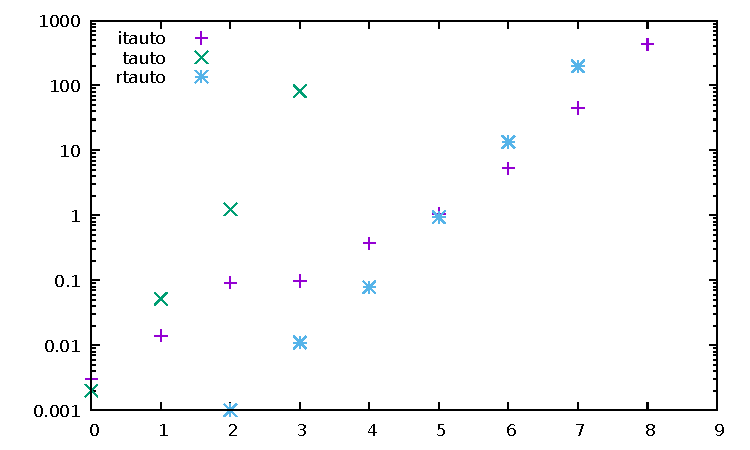
\includegraphics[width=0.45\linewidth]{pdf/pigeon_tac.pdf}}
  \qquad
  \subfloat[\centering Running time of type-checking.]
  {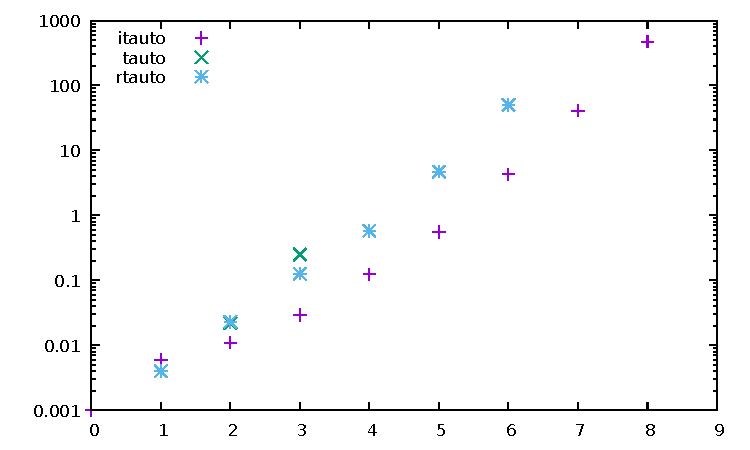
\includegraphics[width=0.45\linewidth]{pdf/pigeon_qed.pdf}}
  \caption{Pigeon Hole for \icoq{itauto}, \icoq{tauto} and \icoq{rtauto}}
  \label{fig:pigeon}
\end{figure}

\end{frame}

\begin{frame}[fragile]{Coq Benchmarks (1/2)}
  Replace all calls of \scoq{tauto}, \scoq{intuition tac}.
%%   \scoq{tac} $\in$ \{\scoq{idtac}, \scoq{assumption},
%%   \scoq{discriminate}, \scoq{congruence}, \scoq{lia}, \scoq{auto},
%%   \scoq{eauto} \}.\\
  \medskip
  
  \scoq{itauto} solves almost every goals but \dots
  \begin{itemize}
  \item Some goals are outside the pure quantifier-free fragment
\begin{minted}{Coq}
Goal true = true <-> (Z -> (False <-> False)).
Proof. Fail itauto congruence.
       itauto (itauto congruence). Qed.
\end{minted}
  \item The leaf tactic (sometimes) needs to be strengthen
    \begin{itemize}
    \item \scoq{idtac} $\to$ \scoq{reflexivity}
    \item \scoq{discriminate} $\to$ \scoq{congruence}
    \end{itemize}
  \end{itemize}

\end{frame}

\begin{frame}[fragile]{Coq Benchmarks (2/2)}
  Tested on two consequent developments: CompCert, Bedrock2\\
  (Sucessful runs)
  \bigskip
  
  \begin{tabular}{|l|c|c|c|c|}
    \hline
    & \#goals & \%faster & \%equal & \%slower \\
    \hline
    Bedrock2  & 1621   &   40   &   40    &   20     \\
    \hline
    CompCert  & 924    &   19   &   76    &   5      \\
    \hline
  \end{tabular}
  \bigskip
  
  \begin{itemize}
  \item  For Bedrock2, speed-up of 1.07
  \item  For CompCert, speed-up of 2.8\\
    19\% are solved 20 times faster!
  \end{itemize}

  Benchmarks are encouraging\dots\\
  Careful implementation is key\dots
  
\end{frame}

\section*{Conclusion}

\begin{frame}{Related Work}
  \begin{itemize}
  \item External SMT provers \emph{e.g.} SMTCoq, SledgeHammer\\
    classic logic, not extensible, much faster
  \item Reflexive (classic) SAT solver in Coq [Lescuyer \& Conchon, 2008]
    \begin{itemize}
    \item CNF \checkmark
    \item Intuitionistic \xmark
    \item Hash-consing \xmark
    \item Lazy Unit Propagation \xmark
    \item Backjumping \xmark
    \item Theory   \xmark
    \end{itemize}
  \item Formalisation of SAT [Blanchette \& Lammich \& Fleury, 2018]
    \begin{itemize}
    \item 2-watched \checkmark
    \item clause learning \checkmark
    \item imperative \checkmark
    \item Reflexive \xmark
    \item Intuitionistic \xmark
    \item Theory \xmark
    \end{itemize}
  \end{itemize}
  
\end{frame}

\begin{frame}{Conclusion}
  Core of SMT solver
  \begin{itemize}
  \item Hash-consing
  \item CNF
  \item Backjumping
  \item Theory as a tactic
  \end{itemize}
  Missing features
  \begin{itemize}
  \item Clause learning (à la Cdcl)
  \item 2-watched literals 
  \item Imperative arrays
  \item À la Nelson-Oppen theory combination [Coq Workshop] 
  \end{itemize}
  \bigskip
  Try it out \url{https://gitlab.inria.fr/fbesson/itauto}\footnote{Happy user of the Patricia Trie library of Alix Trieu}\\
  \icoq{opam install itauto  (deps coq >= 8.13)}
\end{frame}

%%\begin{frame}{Backup Material}
%%  
%%\end{frame}
%%
%%\begin{frame}[fragile]{Definitional CNF à la Plaisted and Greenbaum}
%%
%%%% This facilitate the proofs: no need to \emph{fresh} literals.
%%
%%\[
%%  \begin{array}{c}
%%    \dfrac{ f = (f_1 \land \dots \land f_n) }
%%    {
%%    \begin{array}{l}
%%      \icoq{AND-}(f) = \{\Lit{f} \to \Lit{f_1}; \dots; \Lit{f} \to \Lit{f_n}\}  \\
%%      \icoq{AND+}(f) = \{\Lit{f_1} \to \dots \to \Lit{f_n} \to \Lit{f} \}
%%    \end{array}}\\\\
%%    \dfrac{ f = (f_1 \lor \dots \lor f_n) }
%%    {
%%    \begin{array}{l}
%%      \icoq{OR-}(f)=\{\Lit{f} \to \Lit{f_1} \lor \dots \lor \Lit{f_n}\}\\
%%      \icoq{OR+}(f)=\{\Lit{f_1} \to  \Lit{f} ;  \ldots ; \Lit{f_n} \to \Lit{f}\}               
%%    \end{array}
%%    }\\\\
%%  \dfrac{ f = (f_1 \to \dots \to f_n \to r) }
%%  {
%%    \begin{array}{l}    
%%      \icoq{IMPL-}(f)= \{\Lit{f} \to \Lit{f_1} \to \dots \to \Lit{f_n} \to \Lit{r}\} \\
%%      \icoq{IMPL+}(f)= \{\Lit{r} \to \Lit{f}\} \cup  \bigcup_{\icoq{is_dec}\ f_i} \{\Lit{f_i} \lor \Lit{f}\}
%%    \end{array}
%%    }
%%  \end{array}
%%\]
%%For \icoq{IMPL+}, if  $\neg \bigwedge_{(\icoq{is_dec}\ f_i)}$, keep the \emph{implication clause}
%%$(\Lit{f_1} \to \dots \to \Lit{f_n} \to \Lit{r}) \to \Lit{f} $.
%%\end{frame}
%%
%%\begin{frame}{Proof in a Nutshell}
%%  Well-formedness
%%  \begin{itemize}
%%  \item The initial formula $f$ is hash-consed\\
%%    (Hash-consing is checked w.r.t \icoq{hm:ptrie LForm})
%%  \item Every literal $l$ is hash-consed
%%    ($l$ is a sub-formula of $f$)
%%  \end{itemize}
%%  \[
%%    \phi_i \in \icoq{hm} \land \psi_i \in \icoq{hm} \Rightarrow \phi = \psi
%%  \]
%%  Soundness of dependencies
%%  \begin{itemize}
%%  \item Each clause $c$ is annotated with a set $d$ of literals
%%    \[
%%      \llbracket c_d \llbracket = \bigwedge_{l\in d} \llbracket l \rrbracket \to \llbracket c \rrbracket
%%    \]
%%  \item Unit propagation creates new clauses
%%    \[
%%  \begin{array}{c}
%%  \dfrac{ d_1 \to p  \qquad d_2 \to (p \to r) }
%%    {d_1 \land d_2 \to r } \qquad
%%  \dfrac{ d_1 \to \neg q  \qquad d_2 \to (q \lor r) }
%%    {d_1 \land d_2 \to r }\\\\
%%  \end{array}
%%\]
%%\end{itemize}
%%
%%\end{frame}
%%
%%\begin{frame}[fragile]{Soundness theorem}
%%  \begin{minted}[escapeinside=\#\#,mathescape=true]{Coq}
%%Definition sound_prover (prover: ProverT) (st: state) :=
%% #$\forall$# g lc d, wf_state st #$\to$# g #$\in$# hconsmap st #$\to$#
%% prover st g = Success (lc,d) #$\to$#
%% (#$\llbracket$#st#$\rrbracket$# #$\to$# #$\llbracket$#st#$\rrbracket^{dep}$# #$\to$# #$\llbracket$#g#$\rrbracket$#) #$\land$# (#$\llbracket$#st#$\rrbracket^{dep}$# #$\to$# #$\llbracket$#d#$\rrbracket$# #$\to$# #$\llbracket$#g#$\rrbracket$#)  #$\land$# #$\bigwedge_{c \in lc}$# #$\llbracket$#c#$\rrbracket$#
%%\end{minted}
%%\bigskip
%%\begin{enumerate}
%%\item The learned clauses are tautologies
%%\item The set of clauses (and their annotations) entails $g$
%%\item The annotations and the necessary literals (also) entails $g$
%%\end{enumerate}
%%
%%  
%%\end{frame}
%% \begin{frame}{Case splitting over a Clause}
%%   \begin{itemize}
%%   \item Intuitionistic 
%%     \[
%%       \dfrac{\Gamma,p_1 \vdash q \qquad \Gamma, p_2 \vdash q}
%%       {\Gamma, p_1 \lor p_2 \vdash q}
%%     \]
%%   \item Classic 
%%     \[
%%       \dfrac{ p_1 \lor \neg p_1 \qquad
%%         \Gamma, \neg p_1 \vdash q \qquad \Gamma, p_2 \vdash q }
%%       {\Gamma, p_1 \to p_2 \vdash q}
%%     \]
%%   \item Classic/Intuitionistic 
%%     \[
%%       \dfrac{ \Gamma, \neg p_1 \vdash \bot \qquad \Gamma, p_2 \vdash \bot}
%%       {\Gamma, p_1 \to p_2 \vdash \bot}
%%     \]
%%   \end{itemize}  
%%   NB: SAT solvers simply branch over literals.
%% \end{frame}





\bibliographystyle{plainnat}
\bibliography{biblio}


\end{document}


%%% Local Variables:
%%% mode: latex
%%% TeX-engine: default
%%% TeX-command-extra-options: "-shell-escape"
%%% TeX-master: t
%%% End:


